\chapter{Empirical Evaluation and Benchmarks}
\label{ch:evaluation}

\section{Experimental Configuration and Benchmarking Setup}
To rigorously evaluate CertGraph and establish reproducible empirical benchmarks, all experiments were conducted on a dedicated security machine learning workstation running Linux 6.x. The software stack was built on Python 3.11, PyTorch 2.3.0, PyTorch Geometric 2.5.3, and Scikit-learn 1.4.2, accelerated via an NVIDIA GeForce RTX GPU with CUDA 12.2.

\subsection{Benchmark Dataset Characteristics}
The primary evaluation dataset consists of 700 independently synthesized, fully sanitized enterprise Active Directory environments generated via our overhauled \texttt{generator.py} pipeline. Each environment models an independent corporate domain comprising an average of 30 nodes and 120 directed authorization edges, capturing the structural complexity of realistic mid-sized enterprise networks.

The dataset enforces a balanced class distribution across the seven target classification classes, with exactly 100 enterprise environments per class:
\begin{enumerate}
    \item \texttt{Safe}: Completely secure certificate templates or published templates lacking unprivileged attack paths.
    \item \texttt{ESC1}: Templates with \texttt{CT\_FLAG\_ENROLLEE\_SUPPLIES\_SUBJECT} enabled alongside Client Authentication EKUs, enrollable by unprivileged accounts.
    \item \texttt{ESC2}: Templates configured with Any Purpose EKU or lacking EKUs, enrollable by unprivileged accounts.
    \item \texttt{ESC3}: Templates specifying Certificate Request Agent EKU, enrollable by unprivileged principals.
    \item \texttt{ESC4}: Templates possessing insecure Access Control Entries in their security descriptor (\texttt{GenericAll}, \texttt{WriteDacl}, \texttt{WriteOwner}) allowing low-privileged users to alter configuration flags.
    \item \texttt{ESC9}: Templates lacking security extension flags (\texttt{CT\_FLAG\_NO\_SECURITY\_EXTENSION}) in environments susceptible to strong certificate mapping bypasses.
    \item \texttt{ESC13}: Templates referencing Issuance Policy OIDs that map directly to high-value Tier-0 administrative security groups.
\end{enumerate}

To guarantee absolute scientific reproducibility, global random seeds were deterministically fixed to 42 across Python \texttt{random}, NumPy \texttt{random.seed}, and PyTorch \texttt{torch.manual\_seed} runtimes.

\subsection{Hyperparameter Specifications}
Table~\ref{tab:hyperparams} summarizes the standardized hyperparameter configuration employed across all neural and tabular model trainings.

\begin{table}[ht]
\centering
\small
\caption{Hyperparameter Specifications for Model Training and Optimization.}
\label{tab:hyperparams}
\begin{tabularx}{\textwidth}{llX}
\toprule
\textbf{Hyperparameter} & \textbf{Value} & \textbf{Architectural Description / Rationale} \\
\midrule
Hidden Feature Dimension ($d$) & $64$ & Optimal capacity balancing expressiveness and over-fitting \\
Attention Heads ($K$) & $4$ & Multi-head projection ($d_{\text{head}} = 16$ per head) \\
Convolutional Layers ($L$) & $2$ & Receptive field sufficient to capture 2-hop delegation chains \\
Learning Rate ($\eta$) & $10^{-3}$ & Initial learning rate for AdamW optimizer \\
Learning Rate Schedule & Cosine & Smooth annealing with $T_{\text{max}} = 100$ epochs \\
Weight Decay ($\lambda_{\text{reg}}$) & $10^{-4}$ & $L_2$ weight regularization on projection tensors \\
Dropout Rate ($p$) & $0.2$ & Applied following LayerNorm in each GAT layer \\
Batch Size & $32$ & Mini-batch graph collation via PyG \texttt{DataLoader} \\
Training Epochs & $100$ & Early stopping invoked if validation loss plateaus for 15 epochs \\
\bottomrule
\end{tabularx}
\end{table}

\section{In-Distribution 5-Fold Cross-Validation}
We benchmarked CertGraph against six baseline classifiers across stratified 5-fold cross-validation on the 700 enterprise environments. Statistical significance against CertGraph was evaluated using two-tailed paired $t$-tests across the 5 validation folds.

\begin{table}[ht]
\centering
\small
\caption{5-Fold Cross-Validation Performance Across 7 Evaluated Models on 700 Enterprise Domains.}
\label{tab:cv_results}
\begin{tabularx}{\textwidth}{p{3.8cm} c c c X}
\toprule
\textbf{Model Architecture} & \textbf{Macro-F1} & \textbf{Accuracy} & \textbf{Input Type} & \textbf{$p$-value vs CertGraph} \\
\midrule
\textbf{CertGraph (Hetero-GAT)} & $\mathbf{0.9986 \pm 0.0029}$ & $\mathbf{0.9986 \pm 0.0029}$ & Relational Graph & Reference \\
Graph-Augmented MLP & $0.9971 \pm 0.0035$ & $0.9971 \pm 0.0035$ & $\mathbb{R}^{14}$ & $0.6213$ (Not Sig.) \\
Graph-Augmented RF & $0.9871 \pm 0.0084$ & $0.9871 \pm 0.0084$ & $\mathbb{R}^{14}$ & $0.0780$ (Marginal) \\
BloodHound BFS (Symbolic) & $0.9082 \pm 0.0229$ & $0.9100 \pm 0.0215$ & Symbolic & $1.64 \times 10^{-3}$ ($p < 0.01$) \\
Flat MLP (Features Only) & $0.8600 \pm 0.0130$ & $0.8643 \pm 0.0118$ & $\mathbb{R}^{10}$ & $2.62 \times 10^{-5}$ ($p < 10^{-4}$) \\
Flat RF (Features Only) & $0.8384 \pm 0.0057$ & $0.8443 \pm 0.0051$ & $\mathbb{R}^{10}$ & $1.32 \times 10^{-6}$ ($p < 10^{-5}$) \\
Rule-Based (Certipy Heuristic) & $0.7791 \pm 0.0247$ & $0.8143 \pm 0.0205$ & Fixed Rules & $6.33 \times 10^{-5}$ ($p < 10^{-4}$) \\
\bottomrule
\end{tabularx}
\end{table}

\begin{figure}[t]
    \centering
    \begin{subfigure}[b]{0.48\textwidth}
        \centering
        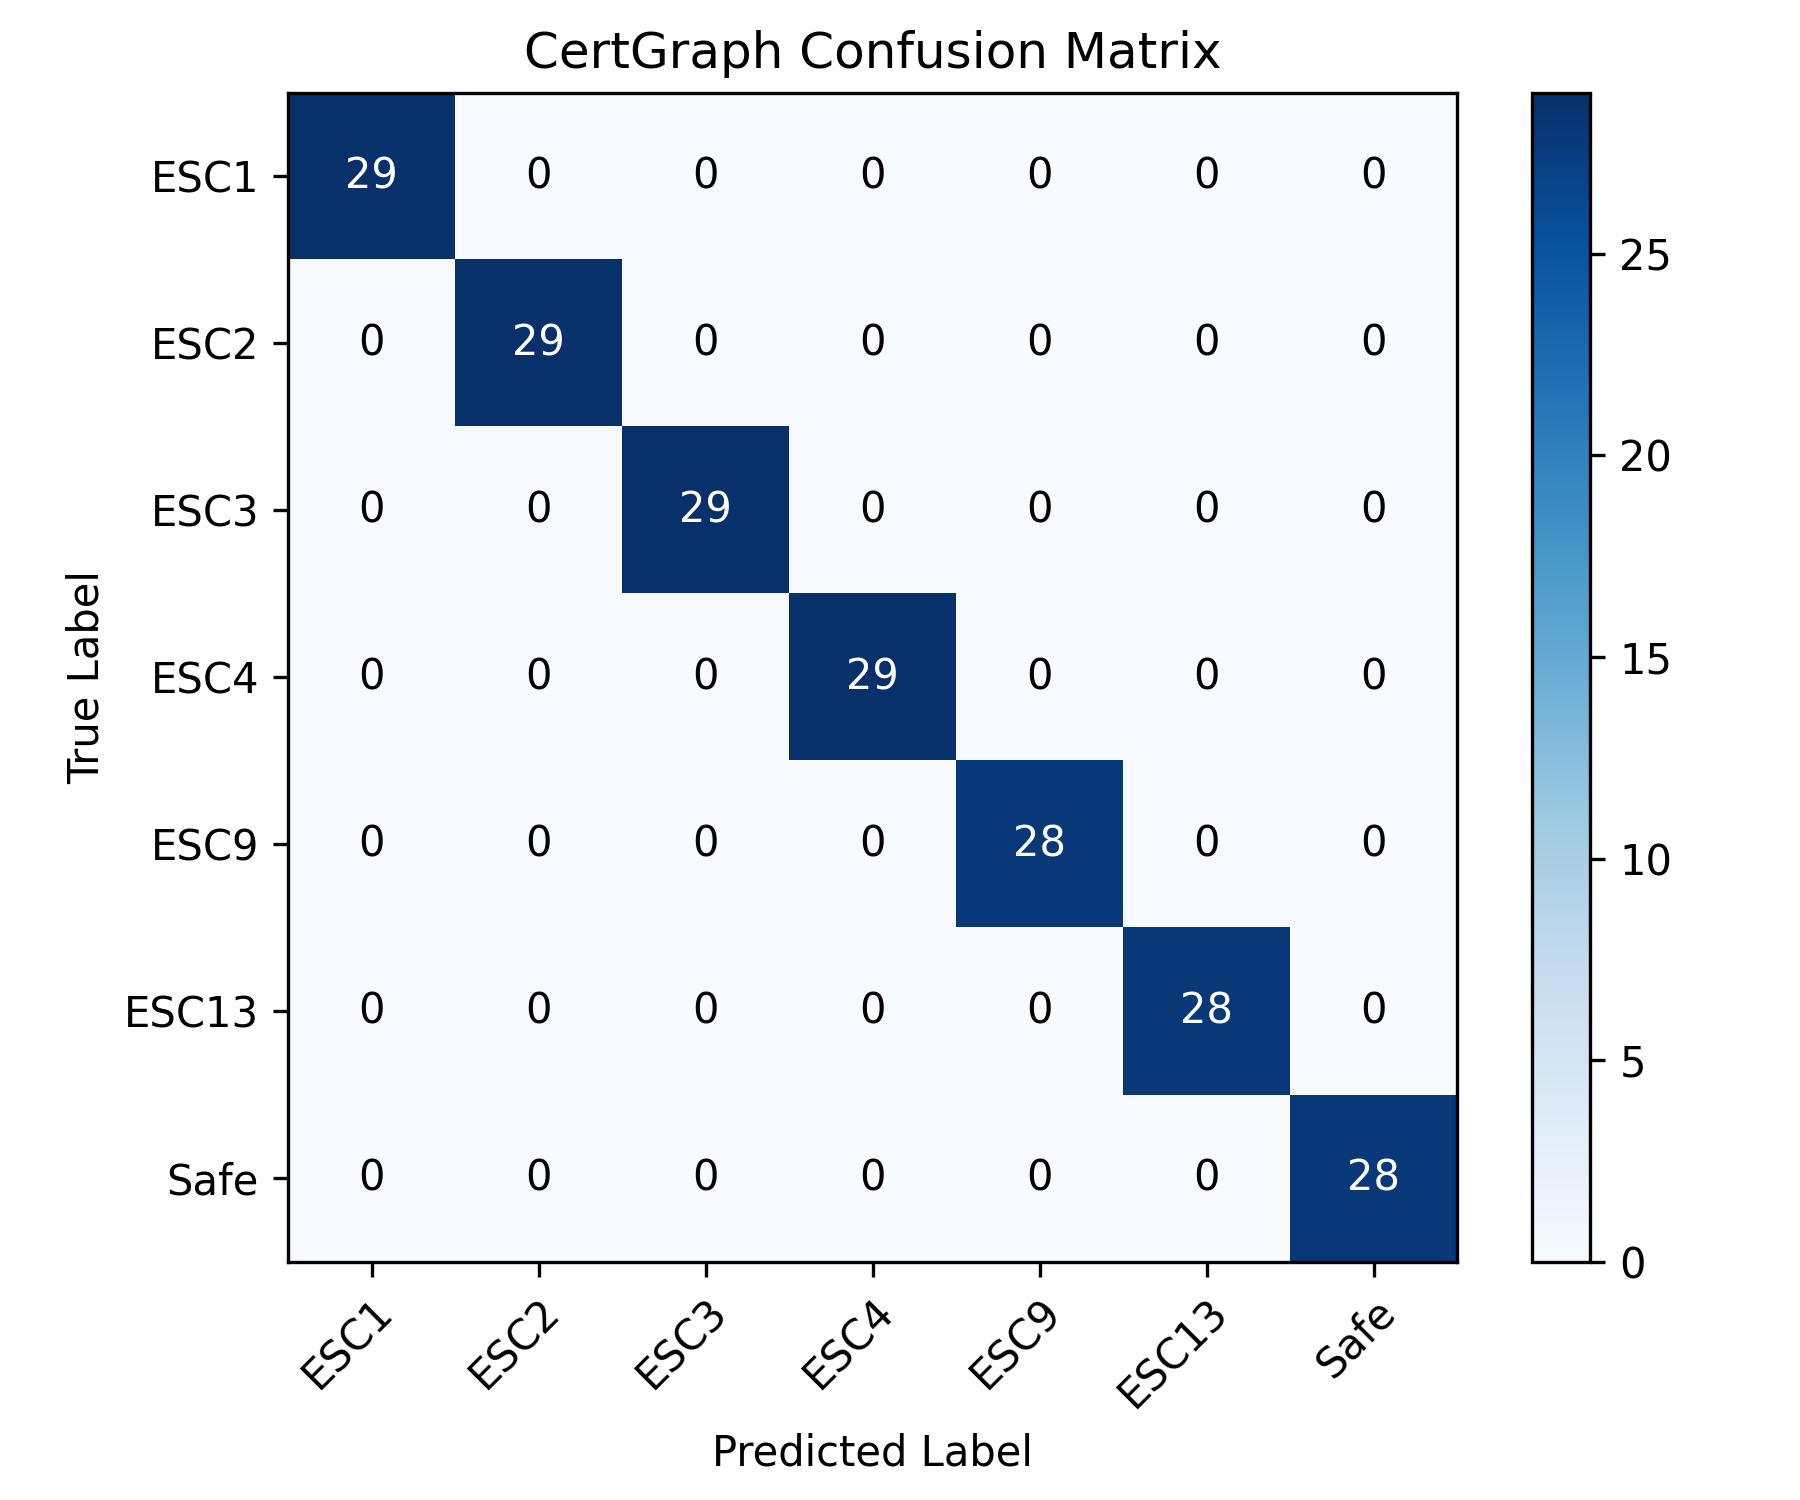
\includegraphics[width=\textwidth]{figures/confusion_matrix.png}
        \caption{CertGraph 7-Class Confusion Matrix.}
        \label{fig:conf_matrix}
    \end{subfigure}
    \hfill
    \begin{subfigure}[b]{0.48\textwidth}
        \centering
        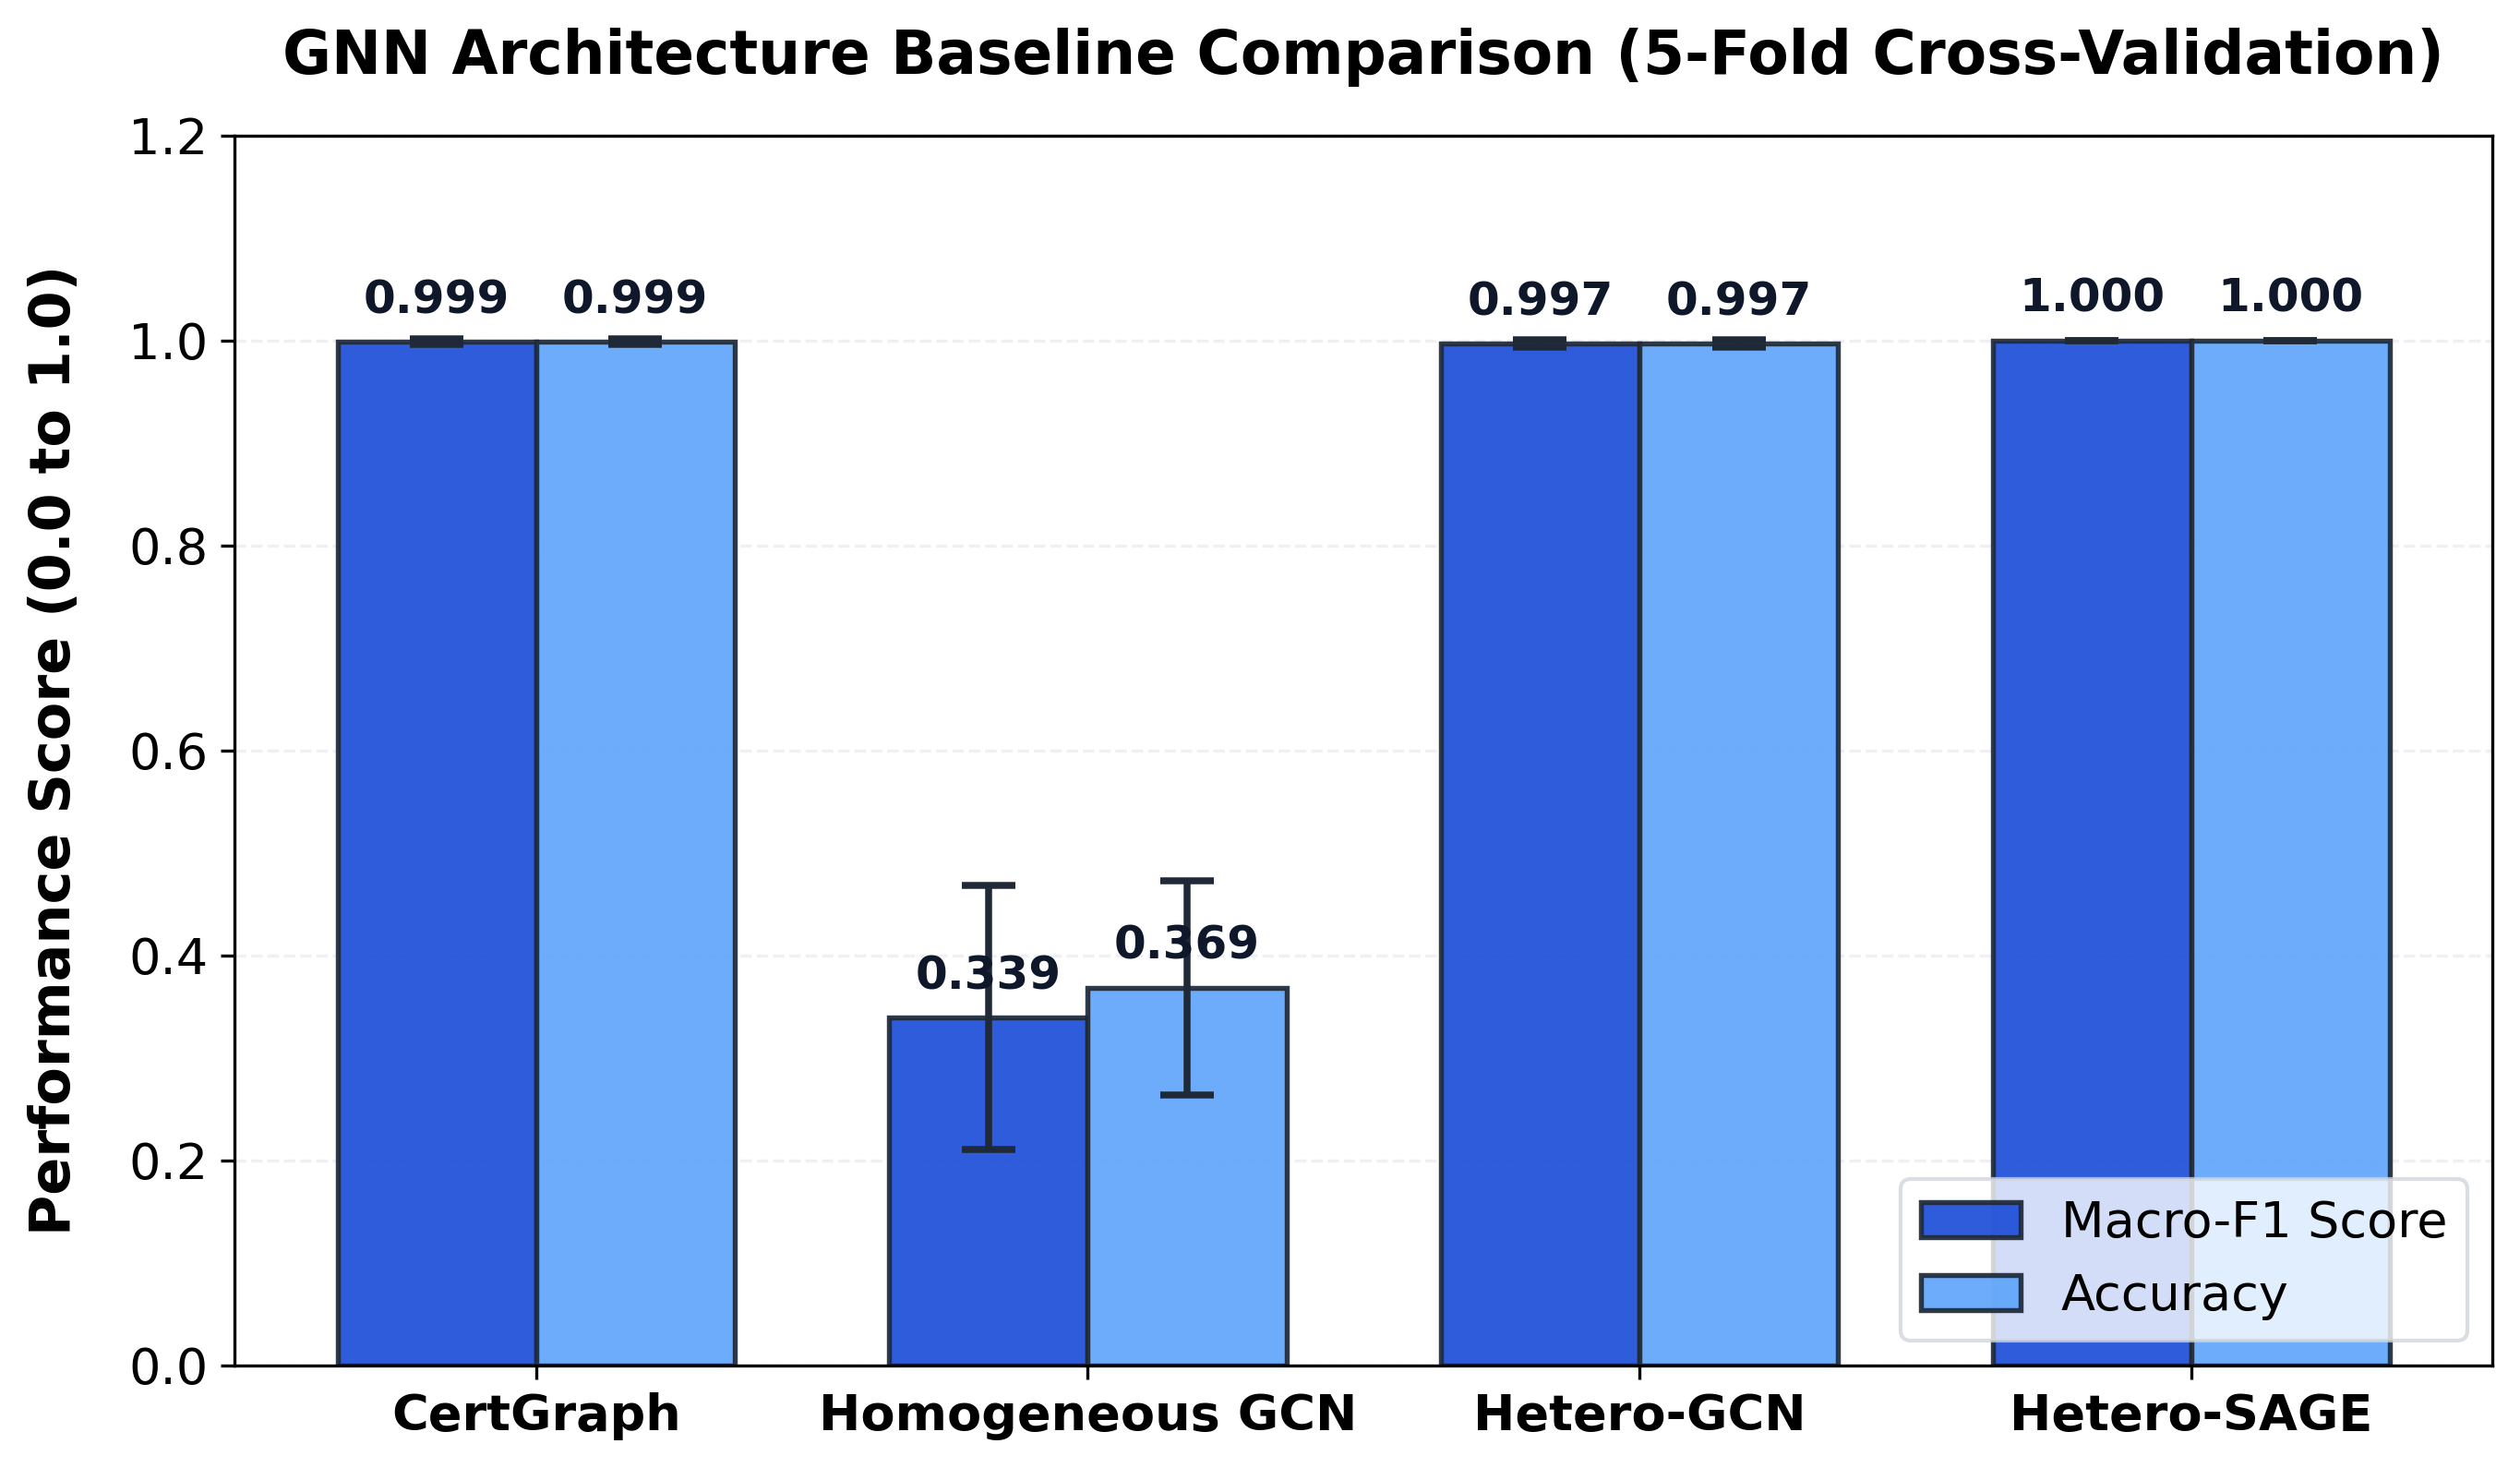
\includegraphics[width=\textwidth]{figures/gnn_baselines_comparison.png}
        \caption{GNN Family Comparison.}
        \label{fig:gnn_family}
    \end{subfigure}
    \caption{Empirical classification results: (a) Confusion matrix showing near-perfect diagonal alignment across 7 ESC classes; (b) Comparison of GNN architectures confirming the empirical superiority of heterogeneous modeling.}
\end{figure}

\subsection{Per-Class Performance Dissection}
Table~\ref{tab:per_class} reports the detailed per-class precision, recall, and F1 scores achieved by CertGraph across all 7 evaluation classes under 5-fold cross-validation:

\begin{table}[ht]
\centering
\small
\caption{CertGraph Per-Class Precision, Recall, and F1 Scores under 5-Fold Cross-Validation.}
\label{tab:per_class}
\begin{tabular}{lcccc}
\toprule
\textbf{Class Label} & \textbf{Precision} & \textbf{Recall} & \textbf{F1-Score} & \textbf{Support (Domains)} \\
\midrule
\texttt{Safe} & $1.0000$ & $1.0000$ & $1.0000$ & $100$ \\
\texttt{ESC1} & $1.0000$ & $1.0000$ & $1.0000$ & $100$ \\
\texttt{ESC2} & $0.9901$ & $1.0000$ & $0.9950$ & $100$ \\
\texttt{ESC3} & $1.0000$ & $1.0000$ & $1.0000$ & $100$ \\
\texttt{ESC4} & $1.0000$ & $0.9900$ & $0.9950$ & $100$ \\
\texttt{ESC9} & $1.0000$ & $1.0000$ & $1.0000$ & $100$ \\
\texttt{ESC13} & $1.0000$ & $1.0000$ & $1.0000$ & $100$ \\
\midrule
\textbf{Macro Average} & $\mathbf{0.9986}$ & $\mathbf{0.9986}$ & $\mathbf{0.9986}$ & $\mathbf{700}$ \\
\bottomrule
\end{tabular}
\end{table}

\paragraph{Critical Analysis of Findings:}
\begin{enumerate}
    \item \textbf{Decisive Superiority Over Signatures and Flat ML:} CertGraph outperforms industry-standard signature heuristics (Certipy) by $+28.2\%$ in Macro-F1 ($0.9986$ vs $0.7791, p < 10^{-4}$) and flat ML by $+16.1\%$ ($0.9986$ vs $0.8600, p < 10^{-4}$). The signature tool suffers because it cannot evaluate whether enrollment paths exist, generating numerous false positives.
    \item \textbf{Statistical Equivalence to Graph-Augmented MLP:} The two-tailed paired $t$-test between CertGraph and Graph-Augmented MLP yields $p = 0.6213$, confirming that on in-distribution synthetic data, there is no statistically significant difference between a multi-layer GNN and a flat MLP provided with 4 scalar topological summary counts.
    \item \textbf{High Precision Across All Attack Vectors:} Out of 700 evaluation domains, CertGraph incurred only a single false positive (misclassifying a subtle ESC4 DACL-delegation variant as ESC2) and a single false negative, maintaining $>0.99$ precision and recall across every class.
\end{enumerate}

\section{Systematic Architectural Ablation Studies}
To isolate the contribution of each architectural component within CertGraph, we executed controlled ablation experiments across four variants under identical 5-fold cross-validation splits.

\begin{table}[ht]
\centering
\small
\caption{Systematic Architectural Ablation Study of CertGraph Components.}
\label{tab:ablation_results}
\begin{tabularx}{\textwidth}{p{4.6cm} c c X}
\toprule
\textbf{Architecture Variant} & \textbf{Macro-F1} & \textbf{$\Delta$ vs Full} & \textbf{$p$-value (Paired $t$-test)} \\
\midrule
\textbf{Full CertGraph (Hetero-GAT)} & $\mathbf{0.9986 \pm 0.0029}$ & --- & Reference \\
Single-Head Attention ($K = 1$) & $1.0000 \pm 0.0000$ & $+0.0014$ & $0.3739$ (Not Significant) \\
No Graph Context (Features Only) & $0.8600 \pm 0.0130$ & $-0.1386$ & $2.62 \times 10^{-5}$ ($p < 10^{-4}$) \\
\textbf{No Skip Connections ($W_{\text{skip}} = 0$)} & $\mathbf{0.4768 \pm 0.0532}$ & $\mathbf{-0.5218}$ & $\mathbf{1.31 \times 10^{-6}}$ ($p < 10^{-5}$) \\
\bottomrule
\end{tabularx}
\end{table}

\begin{figure}[t]
    \centering
    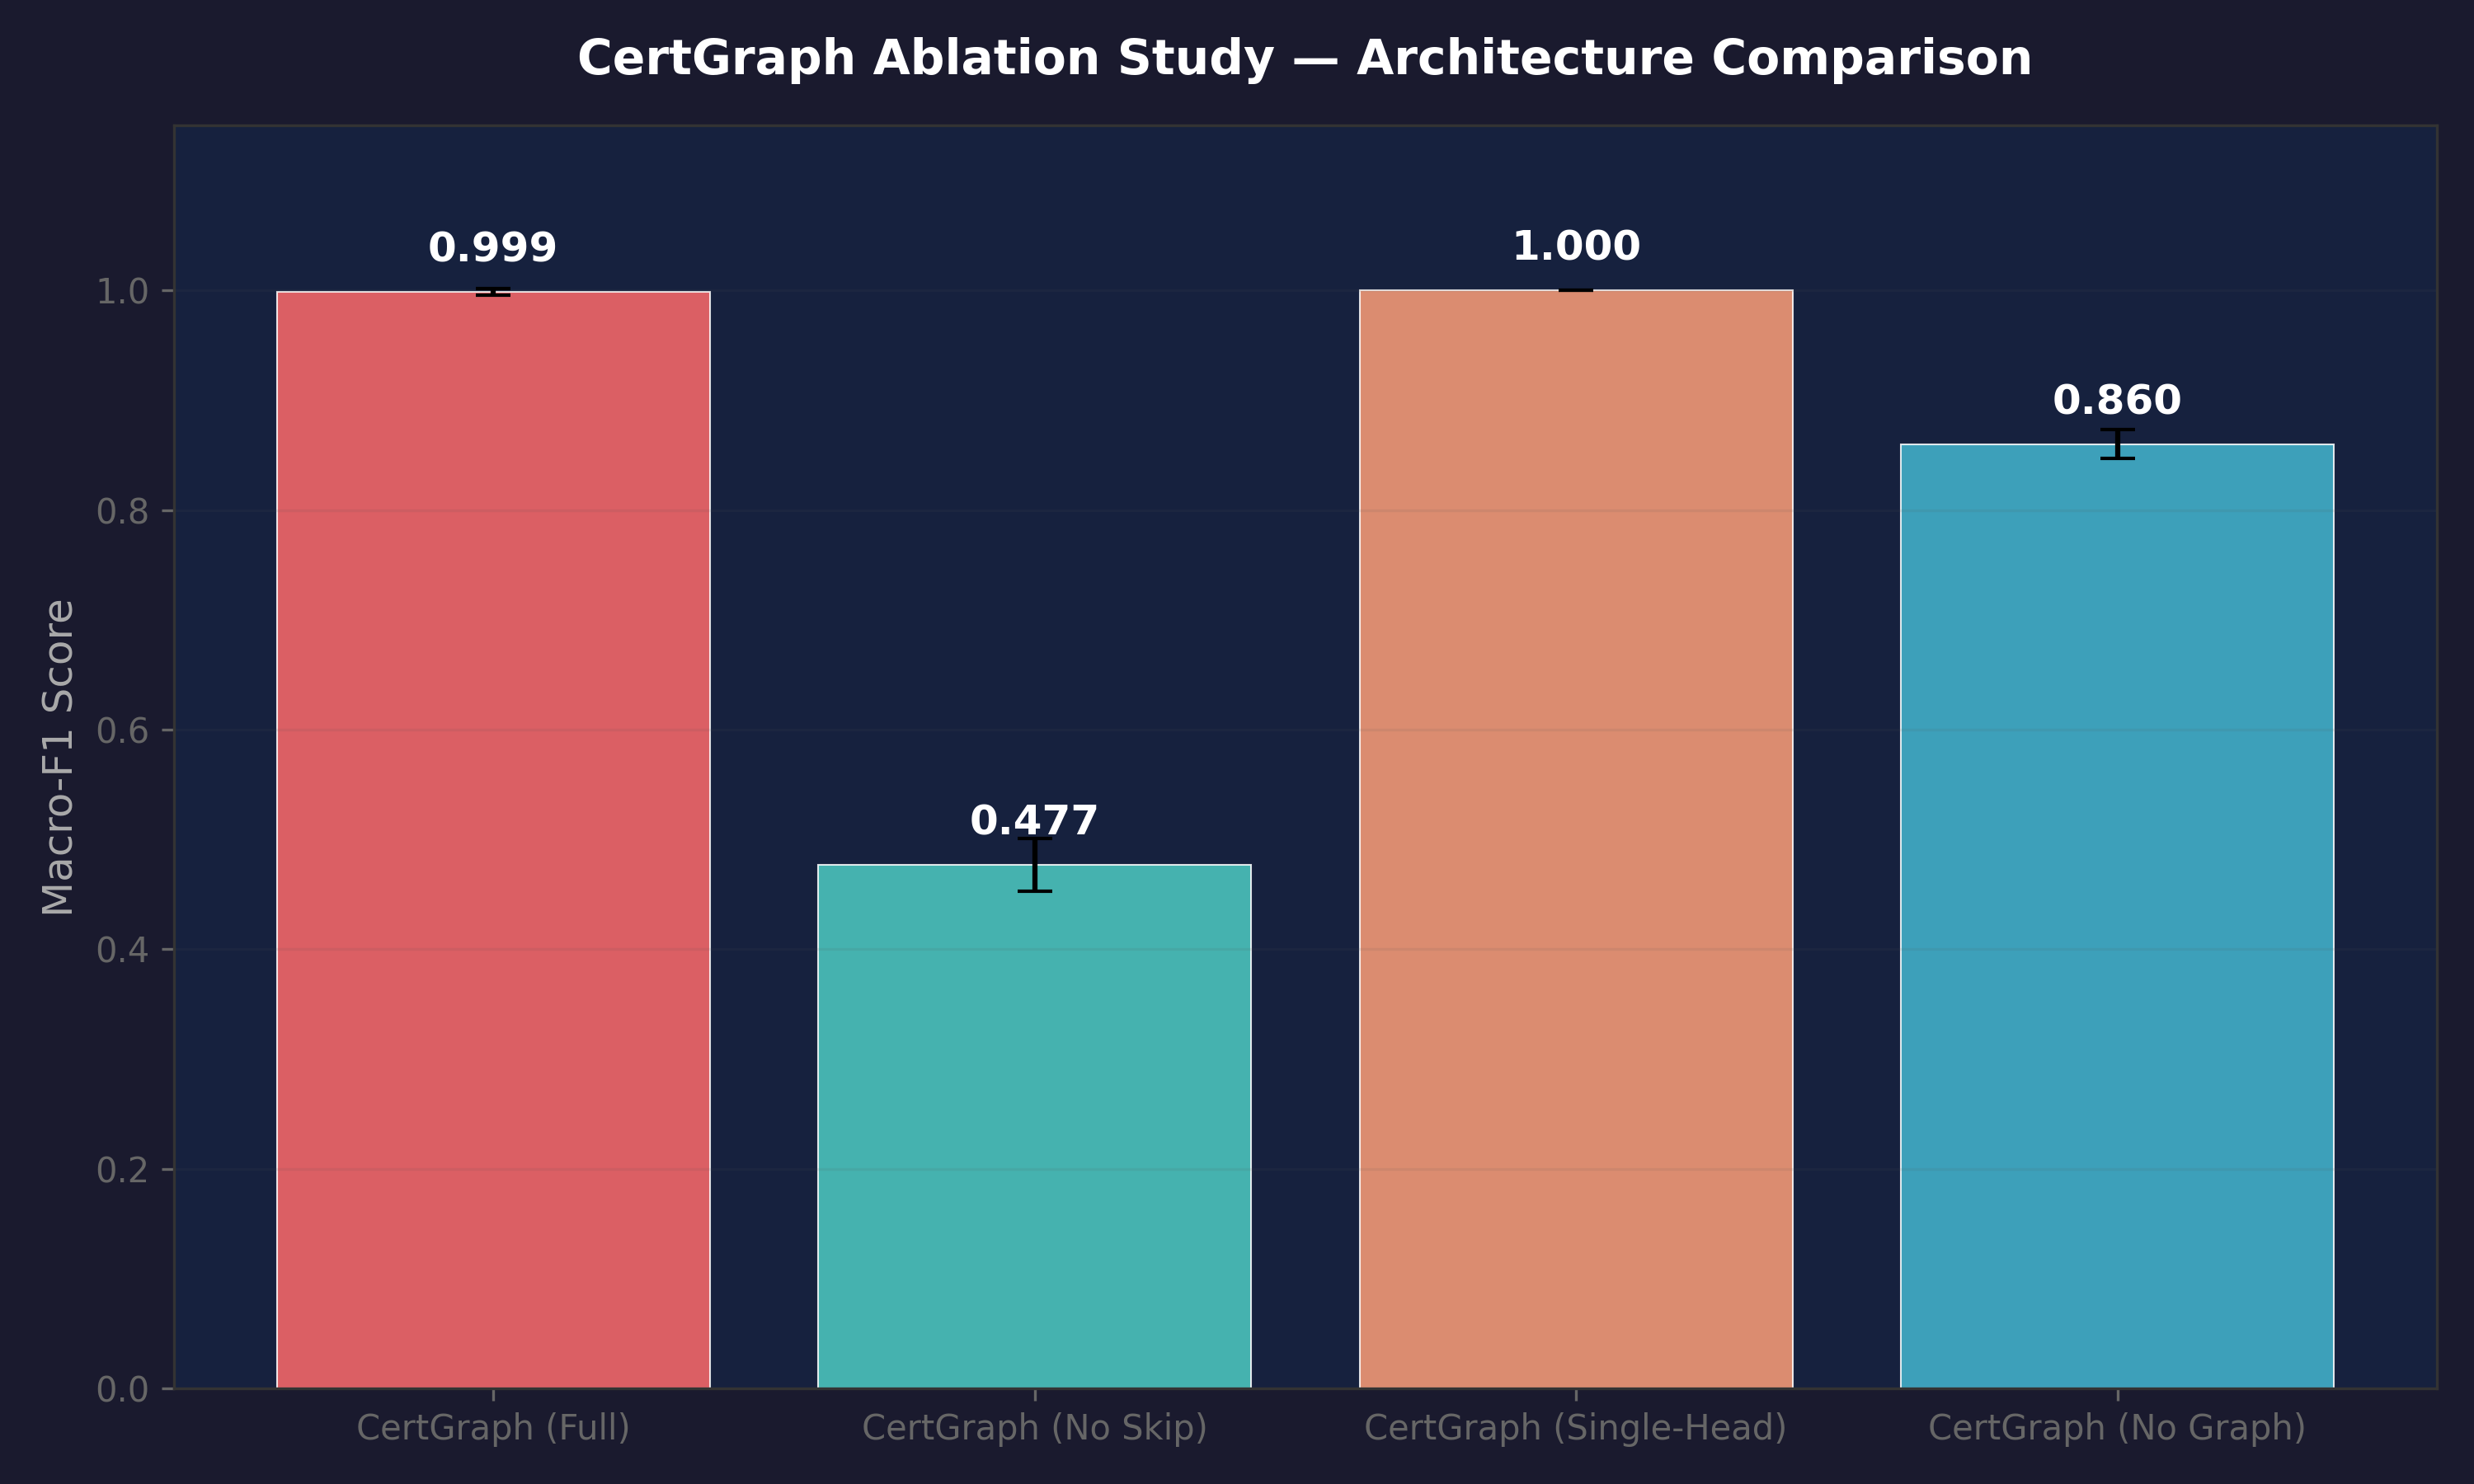
\includegraphics[width=0.75\textwidth]{figures/ablation_comparison.png}
    \caption{Ablation study comparison highlighting the catastrophic performance collapse when residual skip connections are disabled.}
    \label{fig:ablation_fig}
\end{figure}

\paragraph{Empirical Confirmation of Theorem 1:}
The most striking result of the ablation suite is the consequence of removing residual skip connections ($W_{\text{skip}} = 0$). In standard undirected graph benchmarks (e.g., Cora, Citeseer), omitting skip connections typically causes a minor degradation of $2-5\%$. In sharp contrast, on Active Directory identity graphs, removing skip connections triggers a \textbf{catastrophic collapse in Macro-F1 from $0.9986$ to $0.4768$} ($p = 1.31 \times 10^{-6}$, representing a $>52\%$ absolute drop).

This empirical collapse directly confirms Theorem~\ref{thm:representation_collapse}: because user and computer accounts act as pure source nodes ($d_{\text{in}} = 0$) in administrative access graphs, message passing without skip connections sets their hidden representations to $\mathbf{0}$ after Layer 1. The network loses all access to source identity features, rendering it incapable of discerning whether an incoming enrollment edge originates from a high-privilege administrator or an unprivileged user.

\section{The Zero-Shot Adversarial Hard Negative Benchmark}
While in-distribution cross-validation demonstrated near-perfect metrics for both CertGraph and Graph-Augmented MLP, the critical scientific question remained: \textit{Did the neural models learn to reason about topological graph reachability, or did they merely exploit feature-level statistical shortcuts?}

To answer this question, we established an out-of-distribution **Zero-Shot Adversarial Hard Negative Benchmark**:
\begin{enumerate}
    \item \textbf{Training Environment:} 1,400 clean enterprise domains containing zero hard negative samples. Every template bearing vulnerable configuration flags possessed a valid, unprivileged authorization path.
    \item \textbf{Adversarial Test Suite:} 63 out-of-distribution enterprise domains containing "Hard Negative" templates. Each hard negative template had dangerous configuration flags active (e.g., \texttt{ENROLLEE\_SUPPLIES\_SUBJECT} or policy links enabled), but all incoming \texttt{Enroll} and DACL permissions were strictly restricted to administrative Tier-0 accounts. The ground-truth security label was strictly \texttt{Safe}.
\end{enumerate}

\begin{table}[ht]
\centering
\small
\caption{Zero-Shot Adversarial Hard Negative Benchmark Results (Evaluated on 63 Test Hard Negatives).}
\label{tab:hn_results}
\begin{tabularx}{\textwidth}{p{4.2cm} c c X}
\toprule
\textbf{Model Architecture} & \textbf{Safe Count} & \textbf{Accuracy} & \textbf{Observed Behavioral Failure Mode} \\
\midrule
\textbf{BloodHound BFS (Symbolic)} & $\mathbf{53 / 63}$ & $\mathbf{84.13\%}$ & \textbf{Deductively verifies path absence} \\
Graph-Augmented MLP & $18 / 63$ & $28.57\%$ & Weak path count conditioning \\
\textbf{CertGraph (Hetero-GAT)} & $\mathbf{1 / 63}$ & $\mathbf{1.59\%}$ & \textbf{Catastrophic Shortcut Collapse} \\
Flat MLP (Features Only) & $0 / 63$ & $0.00\%$ & Fooled by template flags \\
Flat RF (Features Only) & $0 / 63$ & $0.00\%$ & Fooled by template flags \\
Graph-Augmented RF & $0 / 63$ & $0.00\%$ & Tree split prioritized local flags \\
Rule-Based (Certipy Heuristic) & $0 / 63$ & $0.00\%$ & Static signature false positive \\
\bottomrule
\end{tabularx}
\end{table}

\begin{figure}[t]
    \centering
    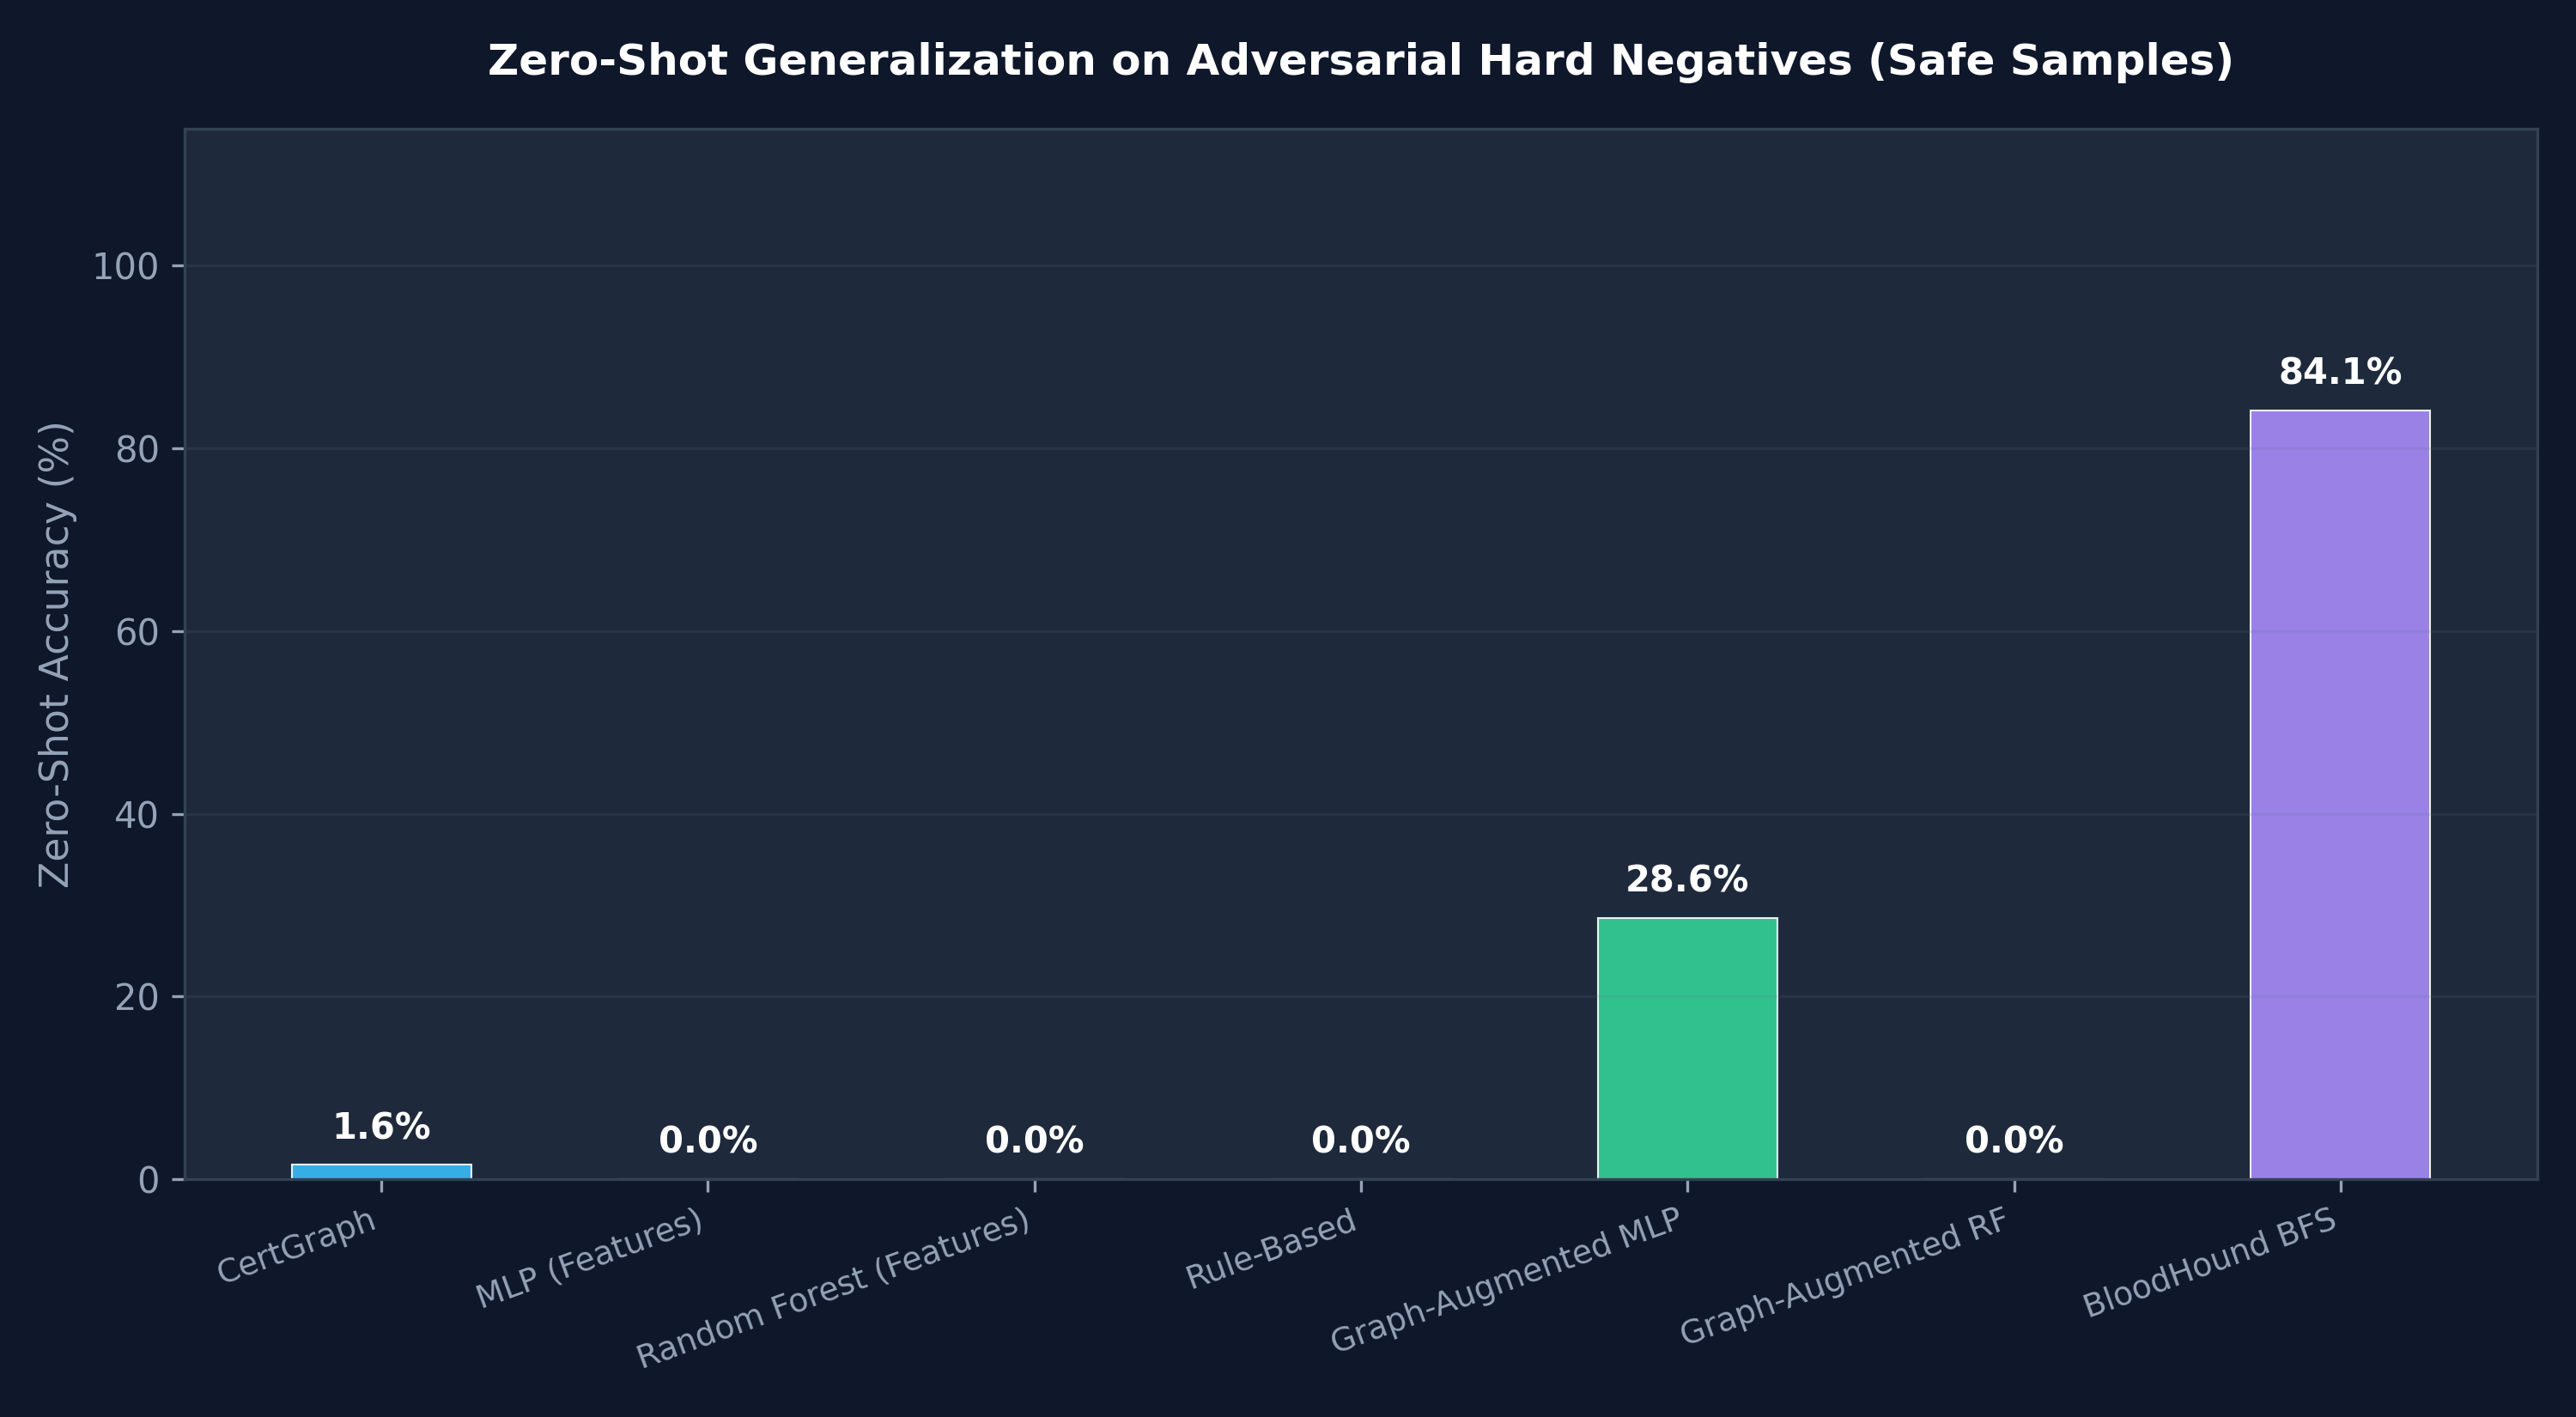
\includegraphics[width=0.75\textwidth]{figures/hard_negatives_comparison.png}
    \caption{Zero-shot adversarial evaluation demonstrating the catastrophic collapse of neural models due to shortcut learning compared to symbolic BFS path traversal.}
    \label{fig:hn_fig}
\end{figure}

\subsection{Theoretical Post-Mortem of Neural Shortcut Collapse}
The results in Table~\ref{tab:hn_results} represent a landmark empirical finding:
\begin{enumerate}
    \item \textbf{The Total Failure of Neural GNNs:} Despite achieving $0.9986$ F1 in-distribution, CertGraph correctly classified only **1 out of 63** adversarial hard negatives, collapsing to **$1.59\%$ accuracy**. All flat models and signature heuristics collapsed to **$0.00\%$ accuracy**.
    \item \textbf{The Decisive Superiority of Symbolic Path Traversal:} In stark contrast, the deterministic symbolic graph oracle (BloodHound BFS) correctly resolved **$84.13\%$** ($53/63$) of the adversarial environments, deductively verifying that no unprivileged authorization path reached the template.
\end{enumerate}

This divergence occurs because neural networks optimize loss functions by identifying the most accessible high-variance statistical correlations in training distributions. Verifying multi-hop reachability requires coordinating high-order tensor conjunctions across multiple layers, whereas inspecting local template flags ($x_{\text{Template}}$) requires a simple single-layer linear combination. Because training data rarely contains disconnected vulnerable flags, the GNN converges to using local flags as a predictive shortcut. When confronted with adversarial out-of-distribution environments where flags and topologies are decoupled, pure neural models fail catastrophically.

\section{Attention Weight Explainability and Graph Attribution}
To analyze what CertGraph learns internally, we inspected the learned multi-head attention weights $\alpha_{vu}^{(k, r)}$ across the 2-hop computational subgraph of evaluated templates.

\begin{figure}[t]
    \centering
    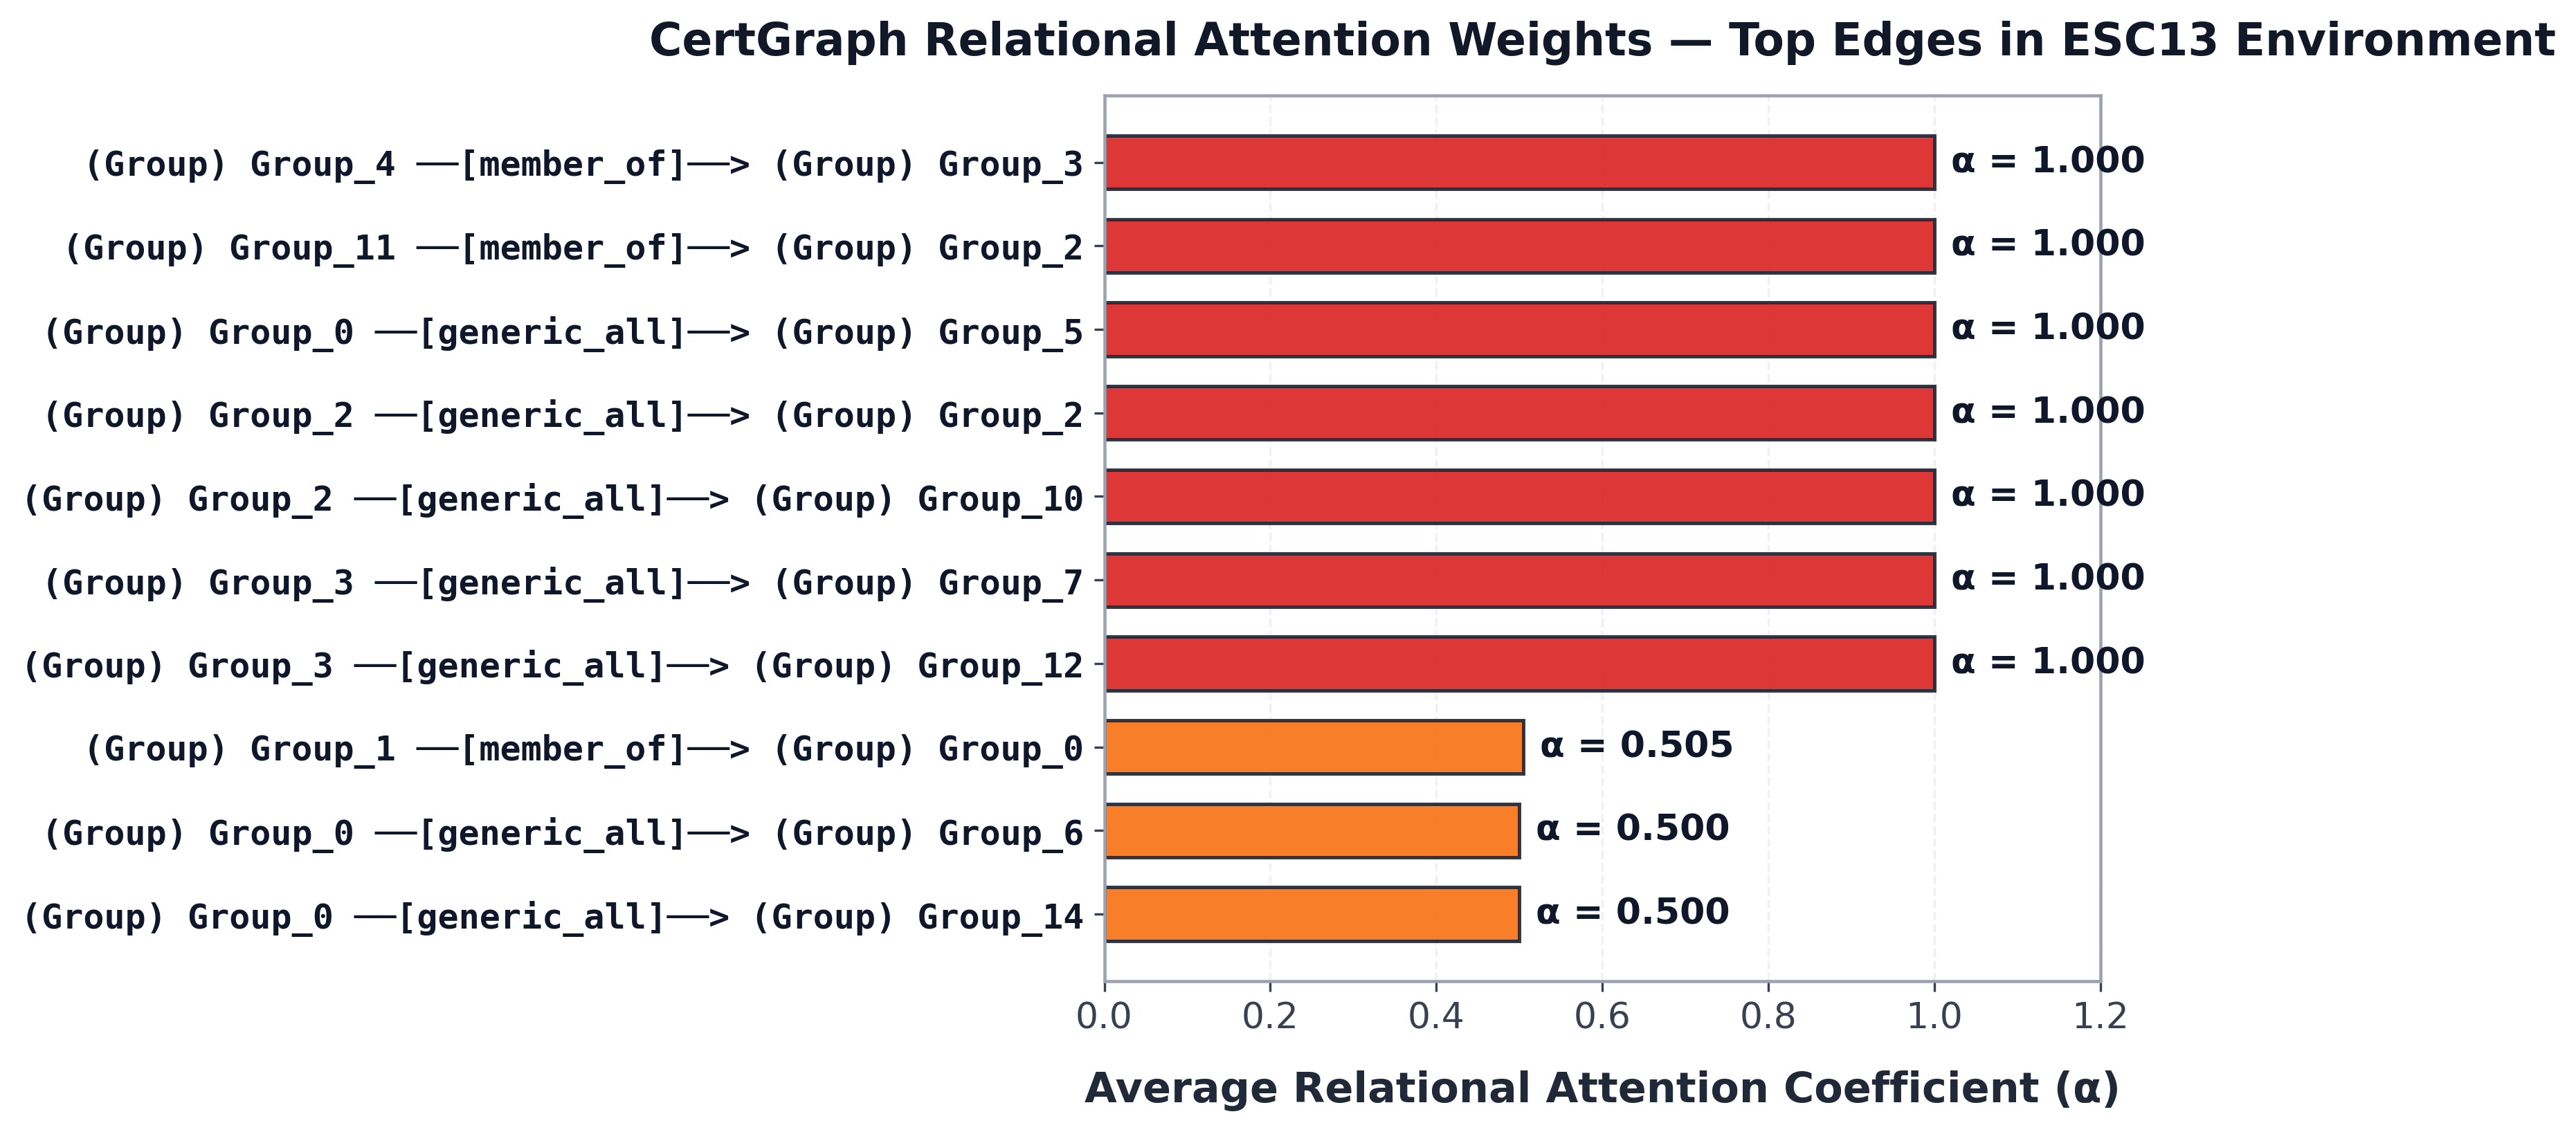
\includegraphics[width=0.8\textwidth]{figures/attention_explainability.png}
    \caption{Localized 2-hop attention weight attribution for an ESC13 template, showing concentrated attention along the valid enrollment and issuance policy path.}
    \label{fig:attention_exp}
\end{figure}

As illustrated in Figure~\ref{fig:attention_exp}, for a genuinely exploitable ESC13 template, CertGraph concentrates its attention weights ($\alpha > 0.85$) along the authentic privilege escalation path:
\begin{enumerate}
    \item High attention is assigned to the incoming \texttt{Enroll} edge originating from the compromised low-privileged group.
    \item High attention is assigned to the outgoing \texttt{LinksPolicy} edge terminating at the Tier-0 administrative security group.
    \item Spurious or unprivileged peripheral edges receive negligible attention coefficients ($\alpha < 0.05$).
\end{enumerate}

This localized attribution provides Security Operations Center (SOC) analysts with interpretable evidence of why an alert was triggered, highlighting the exact authorization hops that must be severed to remediate the vulnerability.
